\documentclass{tufte-book}

\usepackage[utf8]{inputenc}
\usepackage[T1]{fontenc}
\usepackage{amsmath}
\usepackage{amssymb}
\usepackage{xcolor}
\usepackage{booktabs}
\usepackage{microtype}
\usepackage{tikz}
\usetikzlibrary{positioning,calc,shapes.geometric,decorations.pathmorphing,backgrounds,patterns}
\usepackage[most]{tcolorbox}

% ---- palette ----
\definecolor{inkblue}{RGB}{28,60,94}
\definecolor{accentrust}{RGB}{176,86,45}
\definecolor{mossgreen}{RGB}{79,109,74}
\definecolor{softgray}{RGB}{120,120,120}

\hypersetup{colorlinks=true, allcolors=inkblue}

\tcbset{
  boxrule=0.6pt,
  arc=1.5pt,
  left=6pt,right=6pt,top=5pt,bottom=5pt,
  fonttitle=\bfseries\sffamily\small,
}
\newtcolorbox{defbox}[1]{colback=inkblue!5,colframe=inkblue,title=Definition: #1}
\newtcolorbox{insightbox}[1]{colback=accentrust!6,colframe=accentrust,title=Key Insight: #1}

\newcommand{\keyterm}[1]{\textbf{#1}\marginnote{\textcolor{inkblue}{\textit{#1}} --- see running glossary.}}

\title{Networks, Signals, and Small Worlds}
\author{Dr.\ Elena Marsh}
\publisher{Nimbus Academic Press}

\usepackage{hyperref}
\begin{document}

\frontmatter

\maketitle

\newpage
\begin{fullwidth}
\thispagestyle{empty}
\vspace*{2em}
\noindent\textcolor{softgray}{\small Copyright \copyright\ 2026 Elena Marsh. Published by Nimbus Academic Press.
Typeset in the Tufte-\LaTeX\ style. All persons, organizations, and datasets named
in this text are fictional and constructed for pedagogical purposes.}
\end{fullwidth}

\tableofcontents

\mainmatter

\chapter{The Shape of Connection}
\label{ch:shape}

\begin{fullwidth}
\textit{``A network is not a diagram you draw once; it is a question you keep asking
of a system that keeps changing its answer.''} \hfill --- attributed to Dr.\ Elena Marsh,
Vertex Institute for Network Science
\end{fullwidth}

\newthought{Every system worth studying} is secretly a network. The committees that
run a university, the pipes that carry water beneath a city, the citations linking
one paper to the next --- each is reducible to a set of \keyterm{nodes} and the
\keyterm{edges} that join them. This chapter builds the vocabulary needed to talk
about such systems precisely, and then puts that vocabulary to work on a single,
sustained example: the commuter rail network of the fictional city of Meridian.

\begin{marginfigure}
\centering
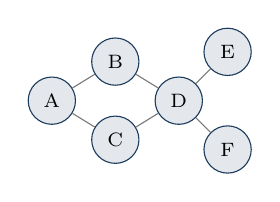
\begin{tikzpicture}[scale=0.62, every node/.style={circle,draw=inkblue,fill=inkblue!12,minimum size=6mm,font=\scriptsize}]
  \node (a) at (0,1.4) {A};
  \node (b) at (1.3,2.2) {B};
  \node (c) at (1.3,0.6) {C};
  \node (d) at (2.6,1.4) {D};
  \node (e) at (3.6,2.4) {E};
  \node (f) at (3.6,0.4) {F};
  \draw[softgray] (a)--(b) (a)--(c) (b)--(d) (c)--(d) (d)--(e) (d)--(f);
\end{tikzpicture}
\caption{A minimal graph: six nodes, six edges. Node D already looks
more important than A --- we will make that intuition precise in
\S\ref{sec:hubs}.}
\label{fig:minimal-graph}
\end{marginfigure}

\section{Nodes, Edges, and the Language of Networks}

\newthought{A graph} $G = (V, E)$ is a set of nodes $V$ together with a set of edges
$E$ connecting pairs of nodes.\sidenote{Mathematicians say ``graph''; the rest of us
say ``network.'' The words are interchangeable in this book, though ``network''
usually implies the edges carry something --- passengers, packets, trust.} An edge
may be \keyterm{directed}, meaning it points from one node to another (a citation,
a one-way street), or \keyterm{undirected}, meaning the relationship is mutual (a
friendship, a shared border).

The \keyterm{degree} of a node is simply the number of edges touching it. In
Figure~\ref{fig:minimal-graph}, node D has degree four while node A has degree two.
This single number --- how many neighbors a node has --- turns out to predict an
enormous amount about how a system as a whole behaves: which nodes to protect,
which to watch, and which to remove if you want to break the whole thing apart.

\begin{defbox}{Clustering Coefficient}
For a node $v$ with degree $k_v$, the clustering coefficient measures what fraction
of $v$'s neighbors are themselves connected:
\[
C_v = \frac{2 \, T_v}{k_v (k_v - 1)},
\]
where $T_v$ is the number of triangles (closed triads) that include $v$. A value of
$C_v = 1$ means every one of $v$'s friends is also friends with every other friend
of $v$ --- a tightly closed circle. A value near $0$ means $v$'s neighbors mostly
do not know one another.
\end{defbox}

Clustering is not a cosmetic statistic. \sidenote{Real social and biological networks
almost always cluster far more than a randomly wired graph of the same size and
density would predict --- this gap is one of the most reliable signatures that a
network is \emph{organic} rather than engineered.} A transit network with high
clustering means nearby stations tend to be cross-connected, which is good for
local trips and bad for long ones; a transit network with low clustering does the
opposite. Neither is wrong --- they are different design philosophies, and Meridian's
planners, as we will see in \S\ref{sec:meridian}, chose deliberately between them.

\section{Small Worlds and Short Paths}

\newthought{In 1967} the psychologist Stanley Milgram asked strangers in Nebraska to
route a letter to a target person in Boston, passing it only through people they
knew personally. The letters that arrived took, on average, about six hops. \sidenote{
The phrase ``six degrees of separation'' outlived the details of Milgram's
methodology, which later researchers criticized on sampling grounds. The rough
finding --- that path lengths in large social networks are surprisingly short ---
has nonetheless replicated many times since, including in email-forwarding and
citation studies.} The finding seemed paradoxical: how can a network of hundreds of
millions of people have such short paths between essentially arbitrary members?

\begin{marginfigure}
\centering
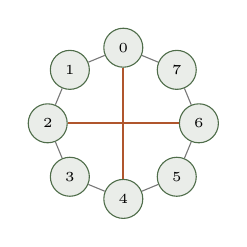
\begin{tikzpicture}[scale=0.6, every node/.style={circle,draw=mossgreen,fill=mossgreen!12,minimum size=4.5mm,font=\tiny}]
  \foreach \i in {0,...,7}{
    \node (n\i) at ({90+\i*45}:1.6) {\i};
  }
  \foreach \i in {0,...,7}{
    \pgfmathtruncatemacro{\j}{mod(\i+1,8)}
    \draw[softgray] (n\i) -- (n\j);
  }
  \draw[accentrust,thick] (n0) -- (n4);
  \draw[accentrust,thick] (n2) -- (n6);
\end{tikzpicture}
\caption{A ring lattice (gray) becomes a small world once a few long-range
shortcuts (rust) are added --- the Watts--Strogatz construction.}
\label{fig:small-world}
\end{marginfigure}

Watts and Strogatz supplied the mechanism in 1998: start with a highly clustered
ring lattice, where each node connects only to its near neighbors, and rewire just
a handful of edges at random into long-range shortcuts (Figure~\ref{fig:small-world}).
Average path length collapses almost immediately, while clustering barely drops.
\keyterm{Small-world networks} therefore combine two properties that naive intuition
says should trade off against one another: tight local structure and short global
reach. Most infrastructure networks --- power grids, road systems, neural wiring,
and, as we will see, transit systems --- sit somewhere on this spectrum, and where
exactly they sit is a design choice with real consequences for cost and resilience.

\section{Hubs, Power Laws, and Fragility}
\label{sec:hubs}

\newthought{Not all nodes} are created equal, and in most real networks the
inequality is extreme. Plot the number of nodes with degree $k$ against $k$ itself
for a road network, and you get something close to a bell curve: most intersections
have three or four roads, almost none have forty. Do the same for an airline route
map, and you get a very different shape.

\begin{figure*}
\centering
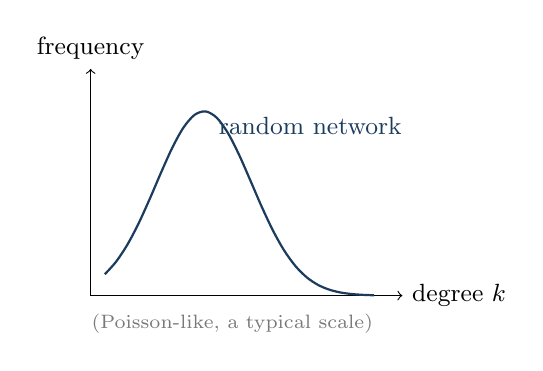
\begin{tikzpicture}[scale=0.9]
  \draw[->] (0,0) -- (4.4,0) node[right,font=\small] {degree $k$};
  \draw[->] (0,0) -- (0,3.2) node[above,font=\small] {frequency};
  \draw[inkblue,thick,domain=0.2:4,smooth,variable=\x]
    plot ({\x},{2.6*exp(-1.1*(\x-1.6)*(\x-1.6))});
  \node[inkblue,font=\small] at (3.1,2.4) {random network};
  \node[softgray,font=\scriptsize] at (2.0,-0.4) {(Poisson-like, a typical scale)};
\end{tikzpicture}
\hfill
\begin{tikzpicture}[scale=0.9]
  \draw[->] (0,0) -- (4.4,0) node[right,font=\small] {degree $k$};
  \draw[->] (0,0) -- (0,3.2) node[above,font=\small] {frequency};
  \draw[accentrust,thick,domain=0.35:4.2,smooth,variable=\x]
    plot ({\x},{2.9/(\x*\x)});
  \node[accentrust,font=\small] at (3.0,1.0) {scale-free network};
  \node[softgray,font=\scriptsize] at (2.0,-0.4) {(power law, no typical scale)};
\end{tikzpicture}
\caption{Degree distributions of two idealized networks. Left: a random (Erd\H{o}s--R\'enyi)
network, where degrees cluster near a mean. Right: a scale-free network, where a
long tail of hubs coexists with a majority of low-degree nodes.}
\label{fig:degree-dist}
\end{figure*}

In a scale-free network the tail follows a power law, $P(k) \sim k^{-\gamma}$, so
there is no ``typical'' node --- some hubs carry far more connections than the
average, and the average itself is a poor description of any particular node.

\begin{insightbox}{The Robustness--Fragility Trade-off}
Scale-free networks are unusually tolerant of random failure --- remove nodes at
random and you will almost always hit a low-degree node that barely matters --- but
unusually vulnerable to targeted attack on their hubs. Remove the top one or two
percent of nodes by degree and the network can fragment entirely. Random networks
show the opposite pattern: no single failure mode dominates, but there is also no
free lunch from redundancy concentrated in a few places.
\end{insightbox}

This trade-off is not an abstraction for the engineers who operate real
infrastructure.\sidenote{The same mathematics describes why a handful of internet
backbone routers matter more to global connectivity than the millions of home
routers behind them, and why epidemiologists target vaccination campaigns at
high-contact individuals rather than distributing doses uniformly at random.} It is,
in fact, exactly the design problem Meridian's transit authority faced when it
expanded its network from four lines to eleven.

\section{Case Study: The Meridian Transit Network}
\label{sec:meridian}

\newthought{Meridian}, a fictional city of 2.1 million people, operates a rail
network that began in the 1950s as a single east--west line and grew, largely
unplanned, into the sprawling system riders navigate today. The transit authority's
2025 modernization review --- carried out jointly with planners from the Vertex
Institute for Network Science --- used exactly the tools built in this chapter to
diagnose why certain stations had become chronic bottlenecks.

\begin{table}[h]
\centering
\small
\begin{tabular}{lrrr}
\toprule
Station & Degree & Clustering $C_v$ & Daily riders (000s) \\
\midrule
Nexa Junction     & 6 & 0.13 & 184 \\
Synapse Crossing  & 5 & 0.20 & 142 \\
Apex Terminal     & 2 & 0.00 & 38  \\
Nimbus Yards      & 3 & 0.33 & 61  \\
Vertex Central    & 7 & 0.10 & 211 \\
\bottomrule
\end{tabular}
\caption{Interchange metrics for five stations on the Meridian network, 2025 audit.
Nexa Junction and Vertex Central are the network's hubs by degree; note their low
clustering, typical of interchanges that connect otherwise-separate branches.}
\label{tab:meridian-stations}
\end{table}

Table~\ref{tab:meridian-stations} shows the pattern predicted by
\S\ref{sec:hubs}: Vertex Central, the busiest interchange, has both the highest
degree \emph{and} the lowest clustering coefficient in the system --- it connects
branches that otherwise share no other path between them. \sidenote{A single
signal fault at Vertex Central in March 2025 delayed an estimated 340{,}000 rider-trips
across the entire network in one afternoon, a real-world instance of the
targeted-hub fragility described in the Key Insight box above.} By contrast, Nimbus
Yards has modest ridership but the highest clustering coefficient in the table: it
sits inside a tightly-knit cluster of suburban stations that mostly serve each
other and rarely need to reach the rest of the city through any single choke point.

\begin{marginfigure}
\centering
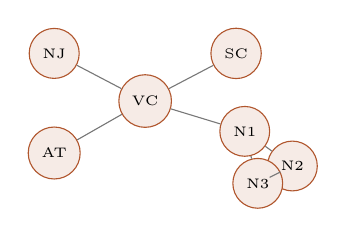
\begin{tikzpicture}[scale=0.55, every node/.style={circle,draw=accentrust,fill=accentrust!12,minimum size=6mm,font=\tiny}]
  \node (vc) at (0,0) {VC};
  \node (nj) at (-2.1,1.1) {NJ};
  \node (sc) at (2.1,1.1) {SC};
  \node (at) at (-2.1,-1.2) {AT};
  \node (ny1) at (2.3,-0.7) {N1};
  \node (ny2) at (3.4,-1.5) {N2};
  \node (ny3) at (2.6,-1.9) {N3};
  \draw[softgray] (vc)--(nj) (vc)--(sc) (vc)--(at) (vc)--(ny1);
  \draw[softgray] (ny1)--(ny2) (ny2)--(ny3) (ny3)--(ny1);
\end{tikzpicture}
\caption{Vertex Central (VC) as articulation point: remove it and the Nimbus Yards
cluster (N1--N3) disconnects entirely from the rest of the map.}
\label{fig:meridian-hub}
\end{marginfigure}

The modernization review's central recommendation followed directly from
Figure~\ref{fig:meridian-hub}: rather than adding capacity \emph{at} Vertex Central,
build one new cross-town connector linking Nimbus Yards directly to Synapse
Crossing. The new edge does not touch the busiest station at all, yet it removes
Vertex Central's status as a single point of failure for roughly 60\% of
suburban riders --- a targeted, low-cost intervention that pure ridership counts,
ignoring network structure entirely, would never have surfaced.

\begin{fullwidth}
\small
\textit{Further reading.} Watts, D.\ J.\ and Strogatz, S.\ H., ``Collective dynamics
of `small-world' networks'' remains the founding text on the ring-lattice
construction in \S1.2. Readers interested in the Meridian audit's full methodology
should consult the Vertex Institute's open technical report, cited in
Appendix~B of this volume.
\end{fullwidth}

\section*{Exercises}
\addcontentsline{toc}{section}{Exercises}

\begin{enumerate}
\item Compute the clustering coefficient of node D in Figure~\ref{fig:minimal-graph}
by hand. Does its value match your intuition about D's role in the graph?
\item Using the degrees in Table~\ref{tab:meridian-stations}, estimate whether the
Meridian network's degree distribution looks closer to the random or the scale-free
curve in Figure~\ref{fig:degree-dist}. What additional stations would you need data
on to answer confidently?
\item Explain, in your own words, why a network can have short average path length
\emph{and} high clustering at the same time. Give one real-world example not
mentioned in this chapter.
\item The transit authority considered a second option: doubling capacity on the
existing Vertex Central interchange rather than building the Nimbus--Synapse
connector. Using the robustness--fragility trade-off, argue for or against this
alternative.
\item \textbf{Challenge.} Suppose Meridian's planners could add exactly one new
edge anywhere in the network to minimize the network's diameter (the longest
shortest path between any two stations). Describe an algorithm --- even an
inefficient one --- for finding that edge.
\end{enumerate}

\end{document}
